\chapter{Analysis}
\label{ch:analysis}
% -----------------------------------------------------------------------------
This project starts with a lot of points to analyze.
From the hardware to the technology used, everything has to be analyzed to be able to make a good project.


\section{Microdispenser $\mu$BoMa}
\label{sec:microdispenser}
% -----------------------------------------------------------------------------
\acrshort{dec} has already done a prototype of the microdispenser $\mu$BoMa but the connected part is missing.
The figure~\ref{fig:analysis:microdispenser:protype} shows the prototype of the microdispenser.

\begin{figure}[ht]
    \centering
    
\includegraphics[width=0.4\textwidth]{img/logo}
    \caption{$\mu$BoMa illustration}
    \label{fig:analysis:microdispenser:protype}\end{figure}

Currently, the dispenser must be connected to an industrial computer using several cables to function.
The goal is to replace all the cables and the industrial computer by a microcontroller that will be connected to the dispenser and provide an interface to control it.


\subsection{Electrical interface}
\label{subsec:interface}
the dispenser has the following pins to be managed.
The figure~\ref{fig:analysis:communication:illustration} shows the type of interface used for each device.

\subsubsection{Rotary valve}
\label{subsubsec:serial}
the dispenser has a rotary valve that can open or close the outputs of the tank.
This valve is actioned by a stepper motor that is controlled by a serial interface.
The standard RS-232~\cite{rs-232} defines the electrical characteristics and timing of the signals but not the protocol used.
This protocol is defined by \acrshort{dec} and more information about can be found in the annexes.

\subsubsection{Pressure sensor}
\label{subsubsec:analog}
To manage the pressure, the microdispenser has a pressure sensor and a regulator.
These two devices are connected to the microdispenser with an analog interface.
These interfaces are using the intensity from 4 to 20mA~\cite{analog} to control the pressure and the volts from 1 to 5~V to read the information.
If the values don't start at 0, it's to detect if the device is connected or not.

\subsubsection{Bubble's detector}
\label{subsubsec:digital}
To detect if there is some bubbles in the tank, the microdispenser has a digital pin.
Now, the tank doesn't have any bubble detector but the sensor still exists anyway.


\section{Communication}
\label{sec:communication}
% -----------------------------------------------------------------------------

To summarize, the microcontroller must be able to communicate with the microdispenser through the electrical interface and with the user.
The figure~\ref{fig:analysis:communication:illustration} shows all the communication medium.

\begin{figure}[ht]
    \centering
    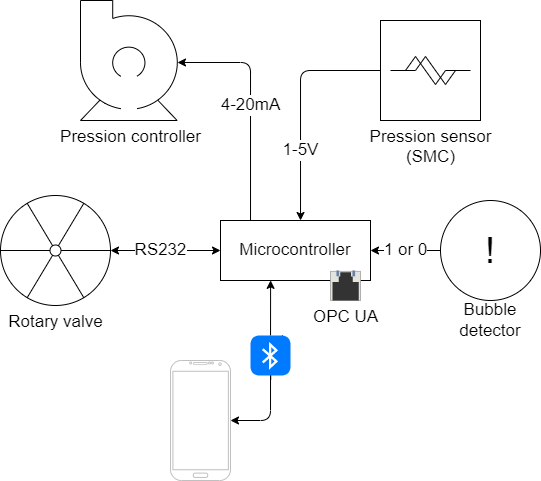
\includegraphics[width=0.8\textwidth]{img/communication.drawio}
    \caption{Communication illustration}
    \label{fig:analysis:communication:illustration}
\end{figure}

The \acrshort{mvp} can be used in different environments and the communication medium must be adapted to each of them.

\subsection{Laboratory}
\label{subsec:laboratory}
In the laboratory environment, the $\mu$BoMa works in standalone.
To order a dispense, the user must use a client application to communicate with the microcontroller.

\subsubsection{Client application}
\label{subsubsec:client}
The client application is a mobile application that uses the Bluetooth to communicate with the microcontroller.
This application is very simple and it only has a text field to enter the volume to dispense and a button to send the order.
The figure~\ref{fig:analysis:communication:laboratory:client} shows the sketch of the application.

\begin{figure}[ht]
    \centering
    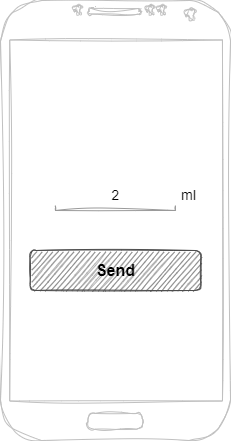
\includegraphics[width=0.3\textwidth]{img/mobapp_sketch.drawio}
    \caption{Client application Illustration}
    \label{fig:analysis:communication:laboratory:client}
\end{figure}

This application is developed with the framework Flutter~\cite{flutter}.
This framework is a cross-platform framework that allows them to develop an application for Android, iOS and web using the code Dart.
It's initially developed by Google and now it's open source.

\subsubsection{Bluetooth}
\label{subsubsec:bluetooth}
The Bluetooth is a wireless technology that allows them to communicate between two devices.
It's a low-power technology that is used in a lot of devices like smartphones, smartwatch and now even more in the laptop.

\subsection{Production}
\label{subsec:ethernet}
When the microdispenser will be used in production, the communication and the power supply will be done with \acrfull{poe}.
This technology allows us to transmit data and power over a single cable.

\subsubsection{OPC UA}
\label{subsubsec:opc}
The communication between the microcontroller and the industrial computer will be done with the \acrfull{opc}~\cite{opc} protocol.
This is a machine-to-machine secure and reliable protocol there is widely used in the industry.
It's a standard protocol oriented service designed to provide a platform-independent.

There is a library for C++~\cite{open62541_2023} that implements \acrshort{opc}.

\section{Microcontroller}
\label{sec:mcu}
% -----------------------------------------------------------------------------
The microcontroller will be the heart of the project.
The chosen one must meet the requirements of the project.
That includes the pins available, the speed, the memory, the availability on the market and the module that can be added to it.
\acrshort{dec} Provide high quality solutions so a top microcontroller can be chosen.

\newpage
\subsection{Requirements}
\label{subsec:requirements}
The table~\ref{tab:analysis:mcu:criteria} is the requirements that the microcontroller must meet to be chosen.
If one of the mandatory cannot be met, the microcontroller will automatically be rejected.

The mandatory criteria required are those where the value is to `Yes'.
In the other case, the number between 0 and 5 shows the relevant of these criteria and this coefficient will be used to compute the score of each microcontroller.


\begin{table}[ht]
    \centering
    \begin{tabular}{|p{2.6cm}|p{2cm}|p{8cm}|}
    \hline
    \multicolumn{1}{|c|}{\textbf{Criteria}} &
      \textbf{Mandatory or Relevant} &
      \multicolumn{1}{c|}{\textbf{Description}} \\ \hline
      \textbf{4-20mA pin}                  & Yes & this pin is to control the pressure in the tank \\ \hline
      \textbf{1-5V pin}                    & Yes & This pin is used to read the pressure from the sensor \\ \hline
      \textbf{Bluetooth/WiFi module}       & Yes & This requirement is needed for the laboratory environment \\ \hline
      \textbf{Ethernet interface}          & Yes & \acrshort{dec} wants to connect their device with a cable due to the stability in a production line \\ \hline
      \textbf{\acrshort{opc}}              & Yes & In the production line environment, the dispenser will communicate with the protocol \acrshort{opc} and the microcontroller must be compatible \\ \hline
      \textbf{Availability on the market} & 5 & It's one of the most important criteria of microcontroller the last years.\\ \hline
      \textbf{Development support}         & 4 & The development provided can be very useful to be productive \\ \hline
      \textbf{Processing power}            & 3 & The microcontroller will probably manage more than one thread at the time \\ \hline
      \textbf{Memory}                      & 2 & Until the program can run without memory errors, this point isn't relevant because the data won't be stored locally \\ \hline
      \textbf{\acrshort{poe}}              & 2 & \acrfull{poe} could be nice to have a cleaner installation. \\ \hline
      \textbf{Learning curve}              & 2 & To accelerate the project, it could be nice if the microcontroller is known \\ \hline
      \textbf{Cost}                        & 1 & \acrshort{dec} would prioritize the quality over the cost \\ \hline
    \textbf{Autonomy} &
      0 &
      The power consumption isn't relevant in this case because the microdispenser will always be connected to something \\ \hline
    \end{tabular}
    \caption{Criteria for the microcontroller}
    \label{tab:analysis:mcu:criteria}
\end{table}

\subsection{Candidates}
\label{subsec:candidates}
The following microcontroller are candidates for the project.
The candidates will be judged with the criteria of the table~\ref{tab:analysis:mcu:criteria}.

\subsubsection{Raspberry pi}
\label{subsubsec:mcu:candidates:pi}
They are a very popular series of single-board computers.
Actually, there is a multiple version and it can be used with Linux distribution.

The Raspberry Pi 4 Model B is the most recent and powerful version~\cite{pi4}.
It's a quad core 64-bit ARM Cortex-A72 processor running at 1.5~GHz and the memory can be 2~GB, 4~GB or 8~GB\@.
This board provides an Ethernet interface, a Bluetooth module and a serial interface.
It's also possible to add an extension to use the 4--20mA pins~\cite{ncdio_2022}.


\subsubsection{STM32}
\label{subsubsec:mcu:candidates:stm32}
STM32 is a series of microcontroller from STMicroelectronics.
There is a multiple version of this microcontroller and it's possible to add an ethernet module and a Bluetooth module.
There are some versions that have a cortex A core, which they are compatible with a Linux this simplifies the usage of the library~\cite{open62541_2023} for the \acrshort{opc}.

\subsubsection{ESP32}
\label{subsubsec:mcu:candidates:esp32}
This is a very popular microcontroller in the \acrfull{iot} world.
It's a dual core 32-bit microcontroller with a clock speed of 240~MHz.
He adds a Bluetooth module and a wifi module and it's also possible to add an ethernet module.
The ESP32 uses a \acrfull{rtos}~\cite{rtos_2023}.

\subsubsection{Arduino}
\label{subsubsec:mcu:candidates:arduino}
Arduino provide microcontrollers and development boards.
The Arduino Uno is the most popular and it's a microcontroller with an 8-bit AVR microcontroller at 16~MHz.
It's possible to add an ethernet shield to use the Ethernet interface and a Bluetooth module.
Arduino use a \acrfull{rtos}~\cite{rtos_2023}.

\newpage
\subsection{Choice}
\label{subsec:choice}
To choice the best microcontroller, the multi-criterion matrix from the table~\ref{tab:analysis:mcu:criteria} will be used.

\begin{table}[ht]
  \centering
  \begin{tabular}{|p{2.6cm}|p{2cm}|c|c|c|c|}
  \hline
  \multicolumn{1}{|c|}{\textbf{Criteria}} &
    \textbf{Mandatory or Relevant} &
    \textbf{Pi} &
    \textbf{STM32} &
    \textbf{ESP32} &
    \textbf{Arduino} \\ \hline
    \textbf{4-20mA pin}                  & Yes & Yes & Yes & Yes & Yes \\ \hline
    \textbf{1-5V pin}                    & Yes & Yes & Yes & Yes & Yes \\ \hline
    \textbf{Bluetooth/WiFi module}       & Yes & Yes & Yes & Yes & Yes \\ \hline
    \textbf{Ethernet interface}          & Yes & Yes & Yes & Yes & Yes \\ \hline
    \textbf{\acrshort{opc}}              & Yes & Yes & Yes & \textbf{No} & \textbf{No} \\ \hline
    \textbf{Availability on the market}  & 5 &   1 & 1 & - & - \\ \hline
    \textbf{Development support}         & 4 &   3 & 2 & - & - \\ \hline
    \textbf{Processing power}            & 3 &   3 & 2 & - & - \\ \hline
    \textbf{Memory}                      & 2 &   3 & 2 & - & - \\ \hline
    \textbf{\acrshort{poe}}              & 2 &   2 & 3 & - & - \\ \hline
    \textbf{Learning curve}              & 2 &   3 & 2 & - & - \\ \hline
    \textbf{Cost}                        & 1 &   1 & 2 & - & - \\ \hline
  \multicolumn{2}{|l|}{\textbf{Total}}    & \textbf{43} & 37 & - & - \\ \hline
  \end{tabular}
  \caption{Choice of the microcontroller}
  \label{tab:analysis:mcu:choice}
\end{table}

The \acrshort{opc} library~\cite{open62541_2023} requires a Linux distribution and only the Pi and the STM32 can be used with a Linux kernel.
There is some work in progress to adapt the library to the \acrshort{rtos} but it's not stable yet.
The Raspberry Pi is better while it offers a better development platform and he can be more adaptable with the different modules.
To reduce the size in a production environment, with can use a NanoPi or a PiCompute.

\subsection{Raspberry PI}
\label{subsec:pi}
To do the \acrshort{mvp}, the simple way is to use a Raspberry Pi 4 Model B\@.
These boards are very popular and they are easy to use.
The figure~\ref{fig:analysis:mcu:pi} shows the Raspberry Pi 4 Model B\@.

\begin{figure}[ht]
  \centering
  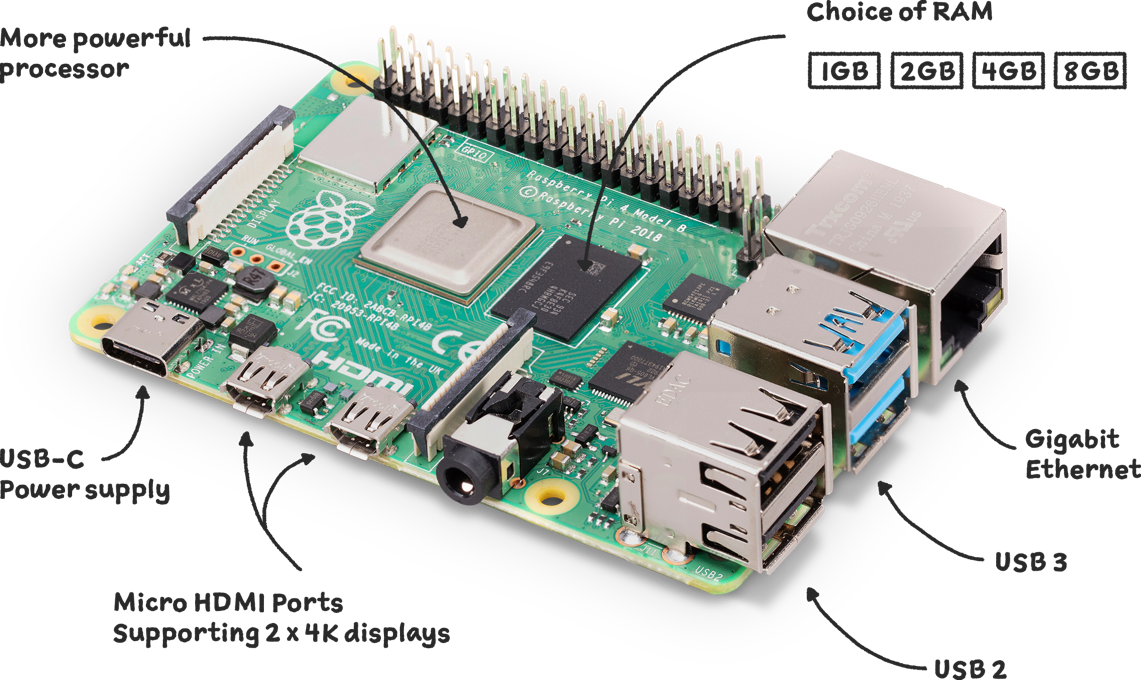
\includegraphics[width=0.6\textwidth]{img/raspberry-pi-4}
  \caption{Raspberry Pi 4 Model B~\cite{raspberryPi4}}
  \label{fig:analysis:mcu:pi}
\end{figure}

To bring on\acrshort{mvp} a production environment, we can use a NanoPi or a PiCompute.
These boards are smaller and they can be more adapted to a production environment.
The advantage of the PiCompute is that it's possible to develop a custom board with the same footprint.
As they are the same processors, the code developed on one can be ported to another.


\subsection{Clickboard}
\label{subsec:clickboard}

Mikroe provides modules named Clickboard~\cite{mikroe-shield}.
These modules are easy to use while they can be plugged on a shield.

\begin{figure}[ht]
  \centering
  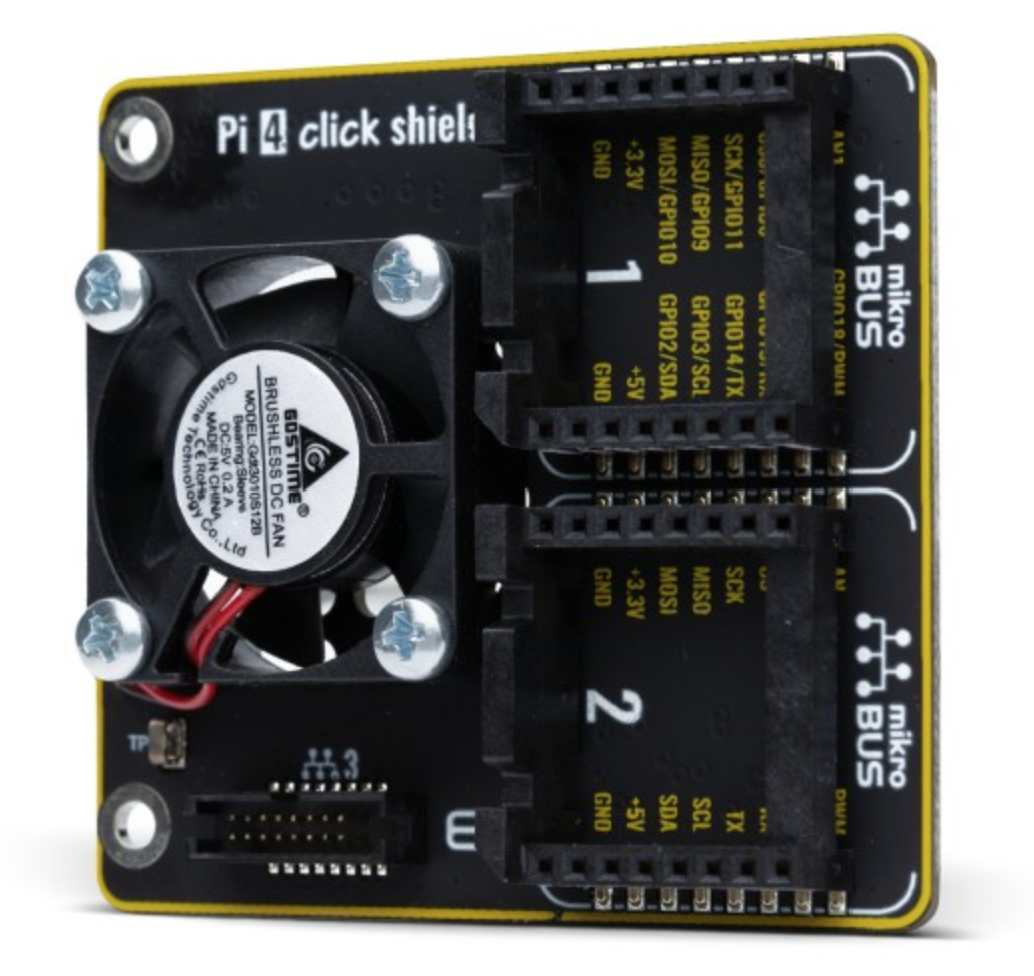
\includegraphics[width=0.4\textwidth]{img/mikroe-shield}
  \caption{Clickboard~\cite{mikroe-shield}}
  \label{fig:analysis:mcu:clickboard}
\end{figure}

The shield on the figure~\ref{fig:analysis:mcu:clickboard} can be plugged on a Raspberry Pi 4 and it has 2 mikroBus slots directly on the board and one that can be plugged with an extension cable.


\subsubsection{RS232}
\label{subsubsec:rs232}
To communicate with the standard RS232~\cite{rs-232}, it's possible to use a USB to RS232 converter but it's not the best solution.
If the final board is a custom board, it's possible there is no USB port.
To avoid this problem, it's possible to use a RS232 clickboard interface.
The figure~\ref{fig:analysis:mcu:rs232} shows this module.

\begin{figure}[ht]
  \centering
  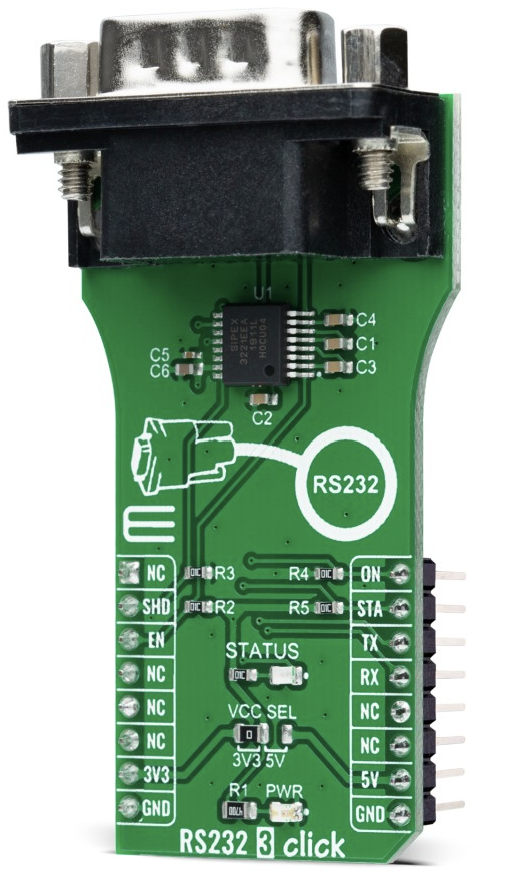
\includegraphics[width=0.15\textwidth]{img/rs232-converter}
  \caption{RS232 to Raspberry Pi~\cite{mikroe-rs232}}
  \label{fig:analysis:mcu:rs232}
\end{figure}

It would be plugged on the clikcboard shield.

\subsubsection{4-20mA}
\label{subsubsec:4-20ma}
To control the pressure in the tank, the microcontroller must provide an intensity between 4 and 20 mA\@.
However, the Raspberry Pi doesn't have this feature, there is a click board that can be used.
The figure~\ref{fig:analysis:mcu:4-20mA} shows this click board that is controlled by the Raspberry Pi through the SPI interface.

\begin{figure}[ht]
  \centering
  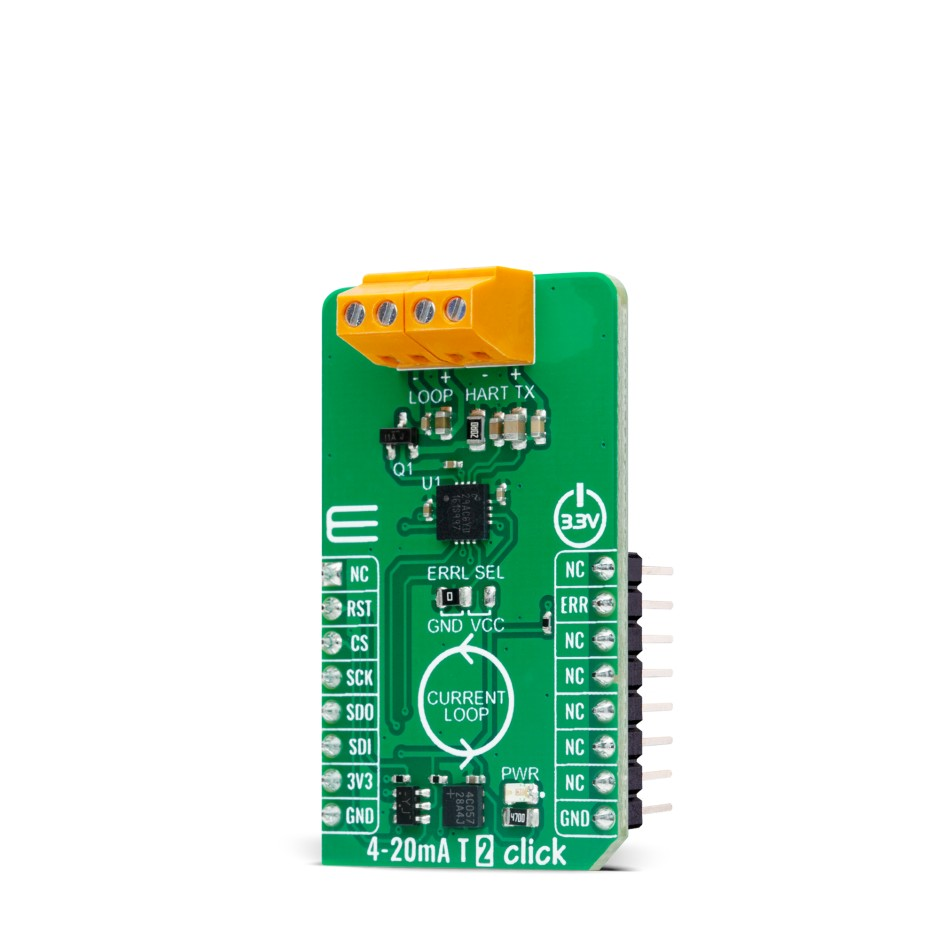
\includegraphics[width=0.3\textwidth]{img/4-20ma}
  \caption{4-20mA T 2 click~\cite{mikroe-420ma}}
  \label{fig:analysis:mcu:4-20mA}
\end{figure}

\subsubsection{1-5V}
\label{subsubsec:1-5v}
To read the pressure in the tank, the microcontroller must read a voltage between 1 and 5~V\@.
Like the 4--20mA, the Raspberry Pi doesn't have this feature and a module is required.
The figure~\ref{fig:analysis:mcu:1-5V} shows a board that can be added to the clickboard shield and controlled by the Raspberry Pi through the SPI interface.

\begin{figure}[ht]
  \centering
  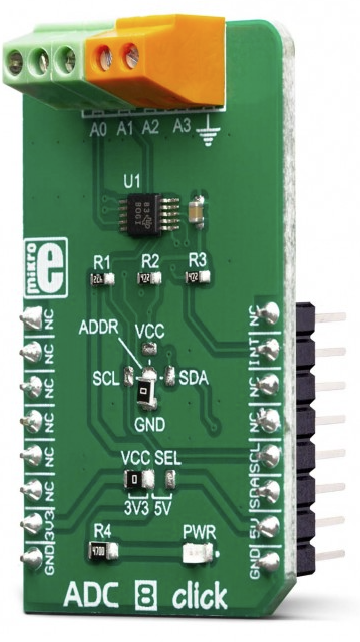
\includegraphics[width=0.15\textwidth]{img/raspberry-1_5V}
  \caption{ADC 1--5V~\cite{mikroe-15v}}
  \label{fig:analysis:mcu:1-5V}
\end{figure}


\subsection{PoE}
\label{subsec:poe}
There is a \acrshort{poe} hat for the Raspberry Pi 4 Model B and the Raspberry Pi 3 Model B/B+.
however, this module isn't relevant for the \acrshort{mvp} but it's interesting for the production environment.
The figure~\ref{fig:analysis:mcu:poe} shows the hat on the Raspberry Pi 4 Model B\@.

\begin{figure}[ht]
  \centering
  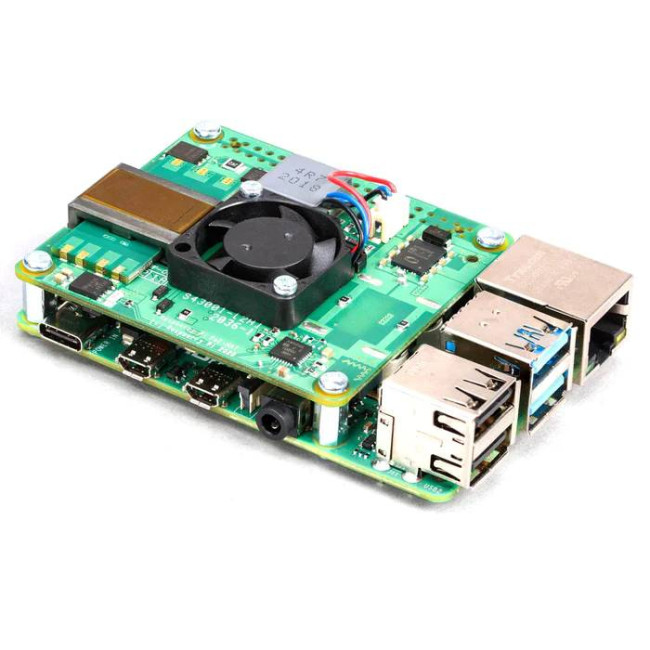
\includegraphics[width=0.3\textwidth]{img/raspberry-poe}
  \caption{PoE HAT~\cite{pi-shop}}
  \label{fig:analysis:mcu:poe}
\end{figure}
\section{Programming language}
\label{sec:lang}
% -----------------------------------------------------------------------------
The programming language is the main tool to produce the \acrshort{mvp}.
It must be chosen carefully because it will be used for the whole project.
To be selected, the language must be able to control the pin of the microcontroller and to communicate with the \acrshort{opc} server.

\subsection{Tiny GO}
\label{subsec:go}
Tiny GO~\cite{tinygo} is a compiler for the language GO~\cite{go} that as for purpose to compile for microcontroller.
Go (aka Golang) is a language created by Google in 2007 and it's now open source.
The purpose is to improve productivity and fit to the multicore networked machines of today.
This language is compiled and statically typed that make it fast and lightweight.
The dependency management and the formatter are built-in that increase the robustness of the project.

\subsection{C}
\label{subsec:c}
C is a language created in 1972.
It's compiled and statically typed and it's very fast.
It's used in many projects and it was very popular until the oriented object language appeared.
Actually, this language is still used in many projects but it isn't easy to learn and it has lack of features like the garbage collector.


\subsection{C++}
\label{subsec:cpp}
C++ is an old object-oriented language created in 1983.
Like GO, it's compiled and statically typed but there is no garbage collector.
The language is very powerful and it's used in many projects.
There is a huge community behind C++ and the embedded programming and the libraries are offently written in C++ and it allows to use C library.

\subsection{MicroPython}
\label{subsec:micropython}
MicroPython~\cite{micropython} is a python implementation for microcontroller.
Python is a high-level language created in 1991.
It's interpreted and dynamically typed and it's very easy to learn.
The language is very popular and there is a lot of libraries available.
This implementation is optimized for microcontroller and it's possible to use it on the Raspberry Pi and many other microcontrollers.

\subsection{Conclusion}
\label{subsec:conclusion}
To complete this case, the best language is C++ because it's the most used language in the embedded world.
The \acrshort{opc} library~\cite{open62541_2023} is written in C++ and there is a variant in other language but the C++ version is the most complete.
\acrshort{dec} They are also using C++ in their project and it's a good point to have a common language.



\section{Development environment}
\label{sec:dev}
% -----------------------------------------------------------------------------
To develop the \acrshort{mvp}, it's necessary to have a development environment.

\subsection{IDE}
\label{subsec:ide}
During the project, the IDE from jetbrains are used.
For the core part, the IDE is CLion and for the client part, that IntelliJ with the Flutter plugin.
To develop directly on the Raspberry Pi from a computer, it's possible to create a Cmake profile that uses a toolchain that is connected to the Raspberry Pi through SSH.

\begin{figure}[ht]
  \centering
  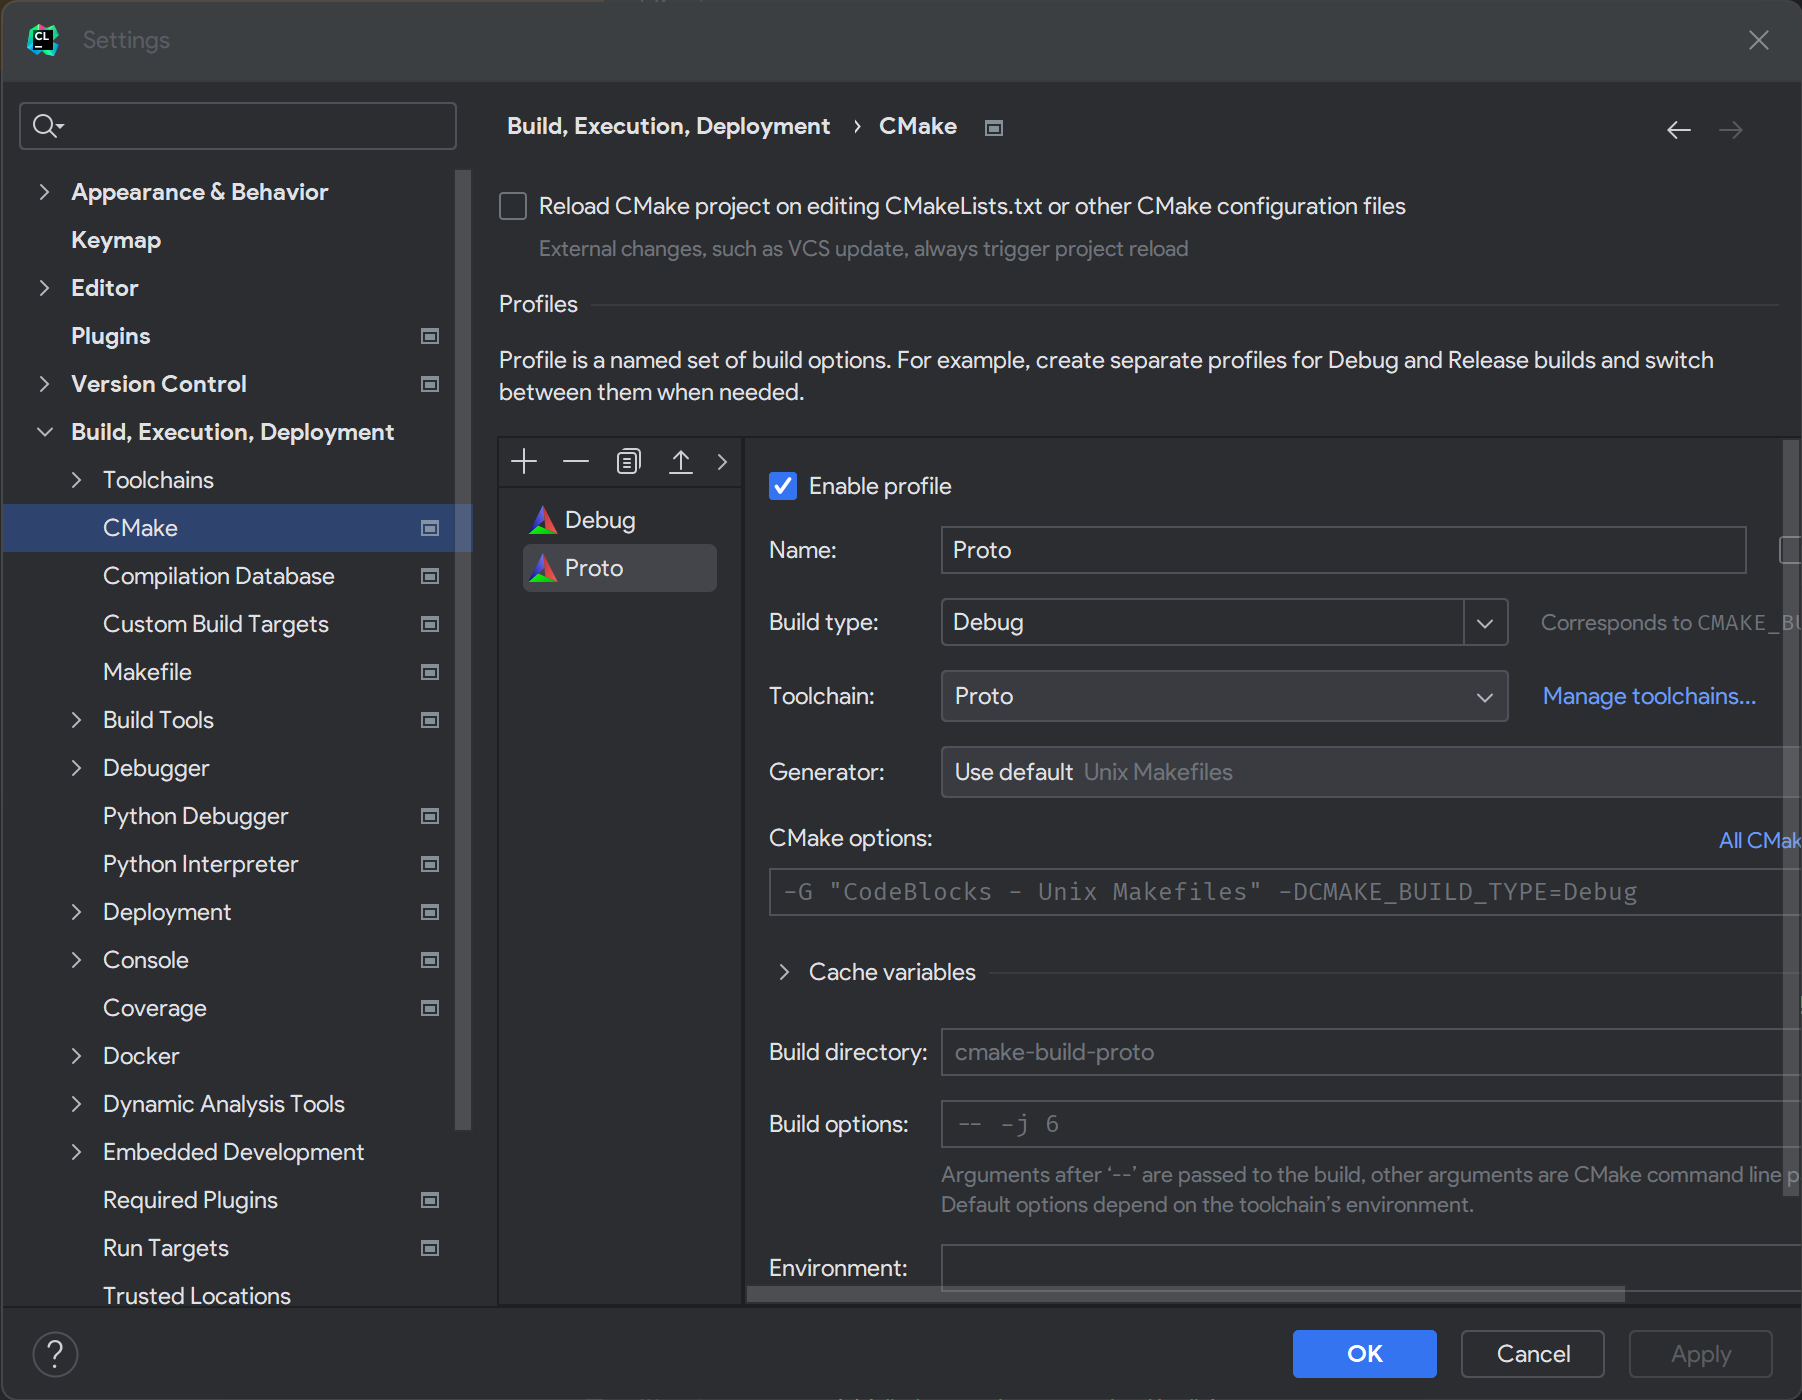
\includegraphics[width=0.75\textwidth]{img/analyze_cmake-profile.png}
  \caption{CMake profile on CLion}
  \label{fig:analysis:dev:clion}
\end{figure}

In the figure~\ref{fig:analysis:dev:clion}, it's possible to see the CMake profile that is used to compile the code on the Raspberry Pi.
The toolchain Proto is a toolchain defined in the Clion settings that is connected to the Raspberry Pi through SSH.

\subsection{Pre-commit}
\label{subsec:pre-commit}

It's recommended to use a pre-commit tool to check the code before committing it.

To install this tool on the computer, it's necessary to have python and install the packages that are mentioned in the file \texttt{requirements-dev.txt}.
Then, to install the hook script, it just needs to run the command \texttt{pre-commit install}.
All these files are at the root of the project.

The following figure \ref{fig:analysis:dev:pre-commit} show what's happened when a git commit is done.

\begin{figure}[ht]
  \centering
  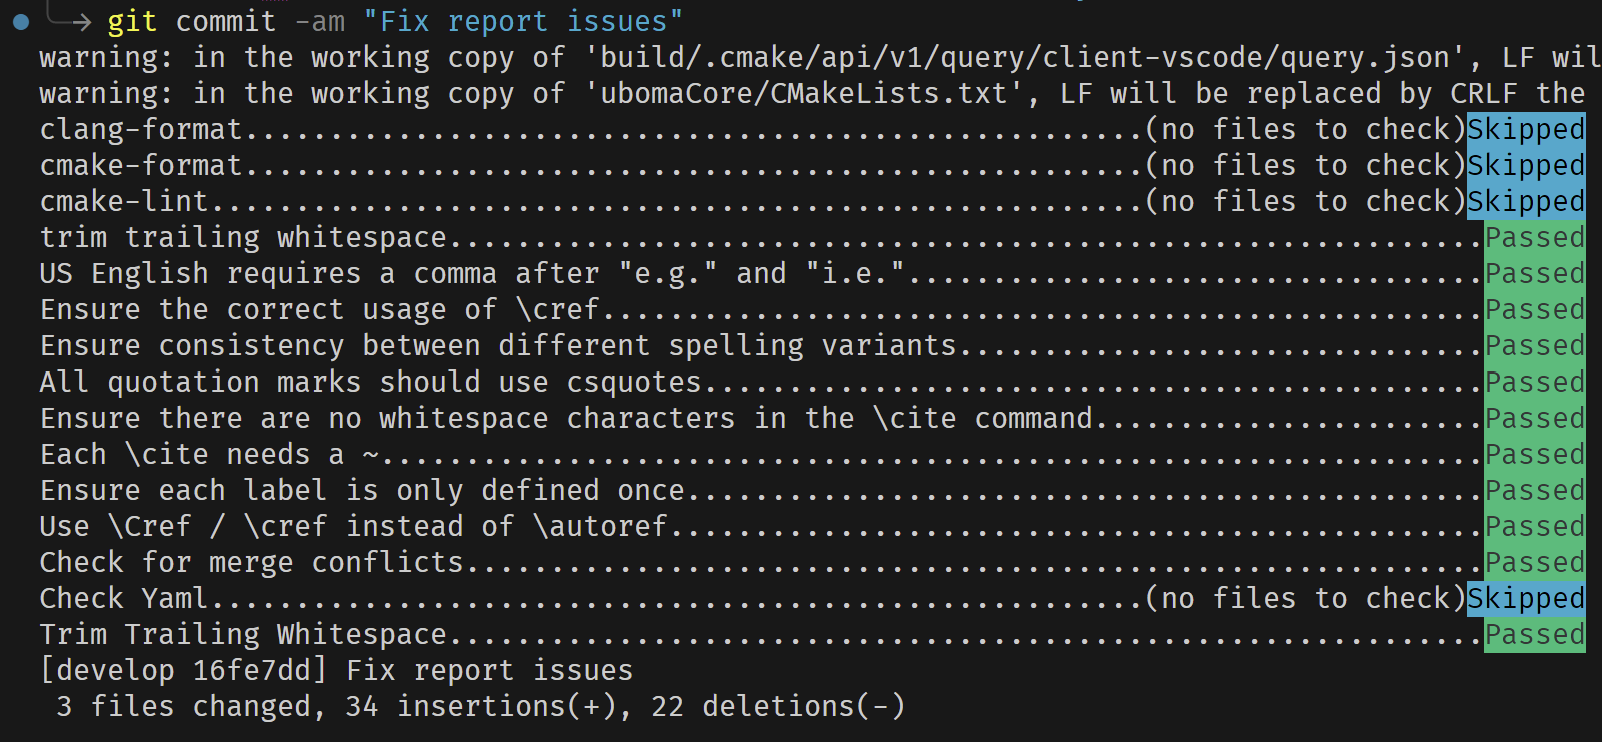
\includegraphics[width=0.75\textwidth]{img/analyze_pre-commit.png}
  \caption{Pre-commit}
  \label{fig:analysis:dev:pre-commit}
\end{figure}

